\chapter{Related Works}
\epigraph{\itshape  A}{-- B}

\startcontents[chapters]
\printmyminitoc{
	%\lipsum[1]
}
% ============================================================
% CHAPTER 2, RELATED WORKS
% Structure: Introduction (with thesis roadmap) -> RSVQA (dense:
% Datasets, Methods) -> Retrieval (Datasets, Methods; CIR/COVR
% focus) -> Captioning (light: Datasets, Models) -> Task-agnostic
% foundation models (consolidated). Entries below match keys in
% related_works_refs.bib
% ============================================================

\section{Introduction}
\label{sec:rw-intro}

The volume of Earth Observation (EO) imagery acquired every day has grown far beyond the capacity of traditional, expert-driven analysis pipelines to exploit it. Natural language offers an accessible interface to this data, allowing non-expert users to query, describe, and search EO archives without specialized remote sensing knowledge. This idea has given rise to a family of vision-language tasks in remote sensing (RS): Visual Question Answering (RSVQA), which answers free-form questions about an image; cross-modal retrieval, which recovers imagery or text based on a query in the other modality; and image captioning, which generates a natural language description of a scene. More recently, these task-specific lines of work have started to converge into general-purpose RS vision-language models and foundation models, capable of handling several of these tasks, and others, within a single architecture.

This thesis engages with this landscape in two stages. It first focuses on RSVQA specifically, contributing three works that progressively extend RSVQA to new data augmentation strategies, segmentation-guided attention, and a new multi-modal dataset and model (TAMMI / MM-RSVQA) combining very high-resolution optical imagery with SAR and multispectral data. Building on this RSVQA foundation, the thesis then explores two directions that connect RSVQA to the other two tasks above: a composed temporal change retrieval contribution (CTCR-RS), which extends composed image retrieval to the temporal, multi-sensor setting; and a multi-task study that trains RSVQA jointly with image captioning and image reconstruction, examining the synergies between these three objectives within a shared model.

This chapter reviews the state of the art accordingly. Section~\ref{sec:rw-vqa} covers RSVQA in depth, the subject of the thesis' first three contributions. Section~\ref{sec:rw-retrieval} covers retrieval, focused on composed image retrieval (CIR), the family of methods CTCR-RS extends to the temporal setting. Section~\ref{sec:rw-captioning} covers captioning, focused on its use in conjunction with RSVQA, since captioning appears in this thesis as one component of the multi-task study rather than as an isolated contribution. Section~\ref{sec:rw-foundation} closes the chapter with task-agnostic RS vision-language models and foundation models, which increasingly cut across all three tasks above and are discussed separately rather than repeated in each task-specific section.

\section{Remote Sensing Visual Question Answering (RSVQA)}
\label{sec:rw-vqa}

\subsection{RSVQA datasets: modality, question diversity, and bias}
\label{sec:rw-vqa-datasets}

RSVQA was introduced by \textcite{lobry2020rsvqa} to allow users to query EO imagery through natural language questions such as "Is there a flood in this image?" or "How many buildings are in this area?". Since then, a large number of datasets have extended the task along three main axes: the image modality considered, the diversity and coverage of the questions, and the overall data volume.

\textbf{Modality of interest.} The image modality is a defining characteristic of a dataset, since it bounds the type of information the answers can be grounded in: optical imagery supports questions about roof color or crop type, multispectral imagery supports questions about vegetation health or water quality, and SAR supports questions about building height or flood extent. The large majority of existing datasets are optical-only, spanning several acquisition scales. UAV-based datasets such as FloodNet-v2~\cite{sarkar2023floodnet} and RescueNet~\cite{sarkar2023rescuenet} offer very fine resolution (0.015m) but limited spatial extent, aimed at post-disaster damage assessment. Satellite-based datasets such as RSVQA-LR~\cite{lobry2020rsvqa} trade resolution (10m, Sentinel-2) for broad, freely available coverage over the Netherlands. Aerial orthophoto datasets sit in between: RSVQA-HR~\cite{lobry2020rsvqa} (0.15m, USGS orthophotos over US cities) and CRSVQA~\cite{zhang2023crsvqa} (0.3m) support more localized, fine-grained questions than satellite data while remaining cheaper to acquire than UAV surveys. HRVQA~\cite{li2024hrvqa} and EarthVQA~\cite{wang2024earthvqa} sit at similarly high resolution (0.08m and 0.3m respectively), the latter specifically targeting relational reasoning over Chinese urban scenes (Nanjing, Changzhou, Wuhan). RSIVQA~\cite{zheng2021rsivqa} instead pools images from five heterogeneous existing datasets (UCM, AID, Sydney, DOTA, HRRSD) spanning 0.15-8m, prioritizing modality diversity over a single consistent acquisition source.

A smaller set of datasets move beyond single-modality optical imagery. CDVQA~\cite{yuan2022cdvqa} takes a bi-temporal image pair as input to support change-detection-style questions rather than static scene description. RSVQAxBEN-MM~\cite{tosato2024can} and OSVQA~\cite{zhao2024textguided} fuse optical and SAR imagery, and this thesis' TAMMI~\cite{boussaid2025tammi} extends this further with a richer multi-modal, multi-resolution design: very high-resolution optical imagery (0.2m, French National Geographic Institute) combined with 10-band multispectral and SAR (VV/VH/Ratio) data from Sentinel-1/2, spanning three distinct French regions (Paris and inner suburbs, Haute-Savoie, Hérault) chosen for urban, mountainous, and coastal diversity respectively. More recently, SAR-only datasets have emerged: SAR-VQA~\cite{cheng2025sartext} and SARLANG-1M~\cite{wei2025sarlang} focus exclusively on SAR imagery, aiming to advance the multi-modal understanding capabilities of instruction-tuned VLMs for SAR interpretation specifically, rather than SAR-optical fusion.

\textbf{Question diversity and coverage.} An ideal dataset would represent the full space of questions an end-user might ask. Fully manual annotation, as used for general-purpose VQA on natural images~\cite{lobry2020rsvqa}, remains rare at scale in RS due to its cost: FloodNet-v2 (43 unique questions), CRSVQA (674 unique questions), and RSIEval~\cite{hu2023rsgpt} (936 samples, purpose-built for evaluation rather than training) are the notable exceptions, but their scale limits the diversity they can offer. Most datasets instead derive questions automatically by filling predefined templates from existing labels or external geographic sources: RSVQA-HR derives questions from OpenStreetMap, while RSIVQA derives them from five source datasets' existing class labels. This approach necessarily bounds the achievable question diversity to what the source data covers; for instance, since OpenStreetMap does not track moving objects, no questions about cars can be generated from RSVQA-HR. TAMMI instead draws on multiple external geographic sources jointly (BD TOPO for geographic features, TRI for flood risk zones, BU20 for urban areas, CLC for land cover, EMA for mountain regions), which broadens the resulting question taxonomy to 21 distinct question types covering presence, quantity, location, classification, and relational analysis.

\textbf{Data volume.} Data volume is a joint consequence of the previous two axes and varies by several orders of magnitude: from a few hundred images (RSIEval) to hundreds of thousands of images and tens of millions of questions (RSVQAxBEN and RSVQAxBEN-MM~\cite{lobry2021rsvqaben,tosato2024can}, both derived from BigEarthNet). Some datasets ask a single question per image (e.g. GLVQA~\cite{GLVQA}), while most, including TAMMI, generate several questions per image, a choice that interacts directly with the answer-balancing strategy discussed below. RSSA~\cite{pang2024h2rsvlm} and VRSBench~\cite{li2024vrsbench} sit at an intermediate point, prioritizing broad visual coverage (1.4M and 29,614 images respectively) over per-image question density.

Table~\ref{tab:rw-vqa-datasets} summarizes the main characteristics of existing RSVQA datasets.

\begin{table}[h]
\centering
\small
\begin{tabularx}{\textwidth}{l X c c c}
\hline
\textbf{Name} & \textbf{Modalities} & \textbf{Resolution} & \textbf{\# Images} & \textbf{\# Questions} \\
\hline
TAMMI~\cite{boussaid2025tammi} & Optical (VHR), MS (10 channels), SAR (VV/VH/Ratio) & 0.2m / 10-20m & 282,852 & 3,162,514 \\
RSVQAxBEN-MM~\cite{tosato2024can} & Optical (RGB), SAR (VV/VH/Ratio) & 10m & 590,326 & 14,758,150 \\
OSVQA~\cite{zhao2024textguided} & Optical, SAR & 1/10m & 6,008 & 1,036,694 \\
RSVQAxBEN~\cite{lobry2021rsvqaben} & Optical (RGB) & 10m & 590,326 & 14,758,150 \\
Chessboard~\cite{tosato2025checkmate} & Optical (RGB) & 10m & 549,488 & 3,123,253 \\
RSIVQA~\cite{zheng2021rsivqa} & Various RGB & 0.15-8m & 37,264 & 111,134 \\
RSVQA LR~\cite{lobry2020rsvqa} & Optical (RGB) & 10m & 772 & 77,232 \\
RSVQA HR~\cite{lobry2020rsvqa} & Optical (RGB) & 0.15m & 10,659 & 1,066,316 \\
FloodNet-v2~\cite{sarkar2023floodnet} & UAV & 0.015m & 2,348 & 10,480 \\
RescueNet~\cite{sarkar2023rescuenet} & UAV & 0.015m & 4,375 & 65,328 \\
HRVQA~\cite{li2024hrvqa} & Optical (RGB) & 0.08m & 53,512 & 1,070,240 \\
EarthVQA~\cite{wang2024earthvqa} & Optical (RGB) & 0.3m & 6,000 & 208,593 \\
CDVQA~\cite{yuan2022cdvqa} & Bi-temporal RGB & 0.5/3m & 2,968 & \\
CRSVQA~\cite{zhang2023crsvqa} & Optical (RGB) & 0.3m & 4,639 & 4,644 \\
RSIEval~\cite{hu2023rsgpt} & Various RGB & & 100 & 936 \\
GLVQA~\cite{GLVQA} & USGS Ortho & 0.3m & 1'500 & 1'500  \\
RSSA~\cite{pang2024h2rsvlm} & Various RGB & 0.08/153m & 1,400,000 & 46,642 \\
VRSBench~\cite{li2024vrsbench} & Various RGB & & 29,614 & 52,472 \\
SAR-VQA~\cite{cheng2025sartext} & SAR & 0.5/15m & 130,000 & 130,000 \\
SARLANG-1M~\cite{wei2025sarlang} & SAR & 0.5/25m & 118,331 & 130,000 \\
\hline
\end{tabularx}
\caption{Existing RSVQA datasets, spanning UAV, aerial, and satellite acquisitions across optical, multispectral, and SAR modalities. Adapted and updated from \cite{boussaidtosato2025tour}.}
\label{tab:rw-vqa-datasets}
\end{table}

\textbf{Biases in RSVQA datasets.} RSVQA, like general-domain VQA, is prone to language bias: models can learn to exploit the skewed distribution of question-answer pairs rather than the image itself, for instance defaulting to "no" for presence questions because the geographic area covered is dominated by absence of the queried object. \textcite{chappuis2025langbias} study this systematically in RS and introduce the $LB_{score}$, which normalizes the prior answer distribution against the theoretical uniform distribution for a given question group, making bias comparable across question groups with very different answer-space sizes (e.g. binary yes/no questions versus open-ended counting questions). Dataset designers address this at the balancing stage of question generation, choosing between reflecting real-world answer distributions (introducing bias but preserving realism), enforcing complete balance (removing bias but also realism), or a compromise: \textcite{lobry2021rsvqaben} apply no balancing, while \textcite{tosato2025checkmate} cap each answer class at the count of its least-frequent class or its median value, and TAMMI applies different balancing rules depending on the answer type while capping the number of pairs per patch. A complementary mitigation strategy is to enforce a different question-answer distribution between training and test splits, e.g. by separating splits geographically (RSVQAxBEN~\cite{lobry2021rsvqaben}) or by drawing the test set from a distinct geographic region with different statistics (RSVQA-HR~\cite{lobry2020rsvqa}).

\subsection{Model architectures for RSVQA}
\label{sec:rw-vqa-methods}

RSVQA architectures typically decompose into four building blocks: image processing, question processing, multi-modal fusion, and answer prediction, as illustrated in Figure~\ref{fig:rw-vqa-pipeline}. This section reviews each in turn, then closes with training strategies that cut across all four. Models that address several of these building blocks at once as part of a larger, task-agnostic foundation model are discussed separately in Section~\ref{sec:rw-foundation}.
\begin{figure}[h]
\centering
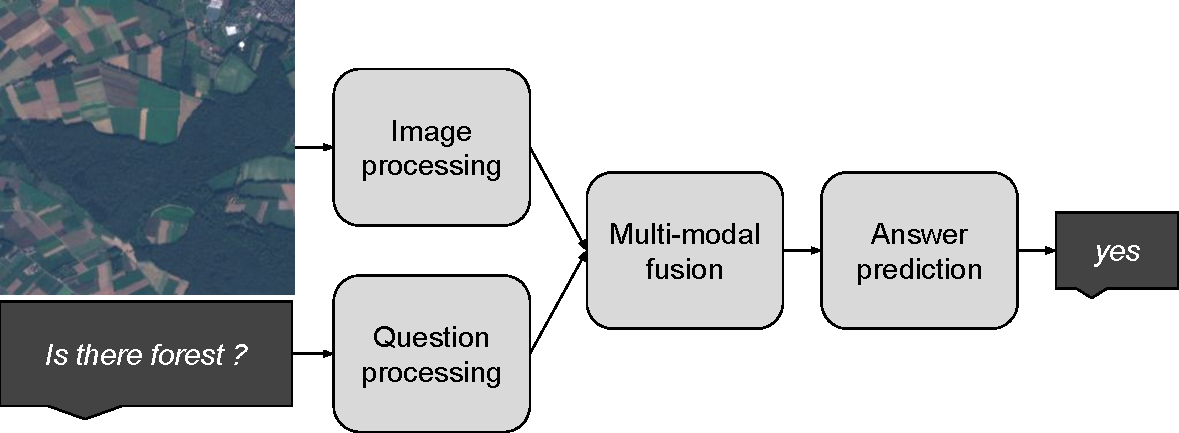
\includegraphics[width=0.85\textwidth]{images/relatedworks/RSVQAoverview.pdf}
\caption{The four building blocks of a typical RSVQA architecture: image and question are processed separately, combined through multi-modal fusion, and passed to answer prediction. Adapted from \cite{boussaidtosato2025tour}.}
\label{fig:rw-vqa-pipeline}
\end{figure}
 
\textbf{Image processing.} The RSVQA baseline~\cite{lobry2020rsvqa} extracts visual features with a frozen ResNet. Later work replaces this with transformer-based image encoders~\cite{bazi2022bimodal} or lightweight adapters that transfer a pretrained encoder's representations to the RSVQA-specific feature space at low cost~\cite{he2024pers}. Several architectures account for the multi-scale nature of RS scenes by explicitly modeling hierarchies across regions and objects, though they do so through different mechanisms: GLVQA~\cite{guo2022glvqa} captures global scene-level and local object-level visual information through two parallel branches whose outputs are fused before answer prediction; SHR-Net~\cite{zhang2023shrnet} instead performs explicit hierarchical spatial reasoning by progressively aggregating features across coarse-to-fine spatial scales; HMGR~\cite{zhang2024hmgr} encodes this hierarchy directly into a graph structure, discussed further under fusion below; SAMFPN~\cite{feng2024samfpn} adapts a feature-pyramid-network-style multi-scale representation combined with contextual attention; and CSCa~\cite{huang2024csca} adds a dedicated cross-modal semantic mapping module to align hierarchical visual features with the question representation. A distinct line of work injects object- or region-level structure directly: \textcite{felix2021crossmodal} use a dedicated object detector as feature extractor, while segmentation-guided attention~\cite{tosato2024segguided,wang2024earthvqanet} uses image segmentation to focus the model's attention on the regions relevant to the question. PAN-RSVQA~\cite{chappuis2025pan} combines several such pseudo-annotation streams (classification, segmentation, detection, generic features) from a vision foundation model into a single multi-task visual encoding. Beyond RGB, \textcite{tosato2025b} fuse optical and SAR features directly as visual input, establishing a baseline for SAR-aware RSVQA.

\textbf{Question processing.} This building block has received comparatively less attention. The baseline uses a Skip-thought RNN~\cite{kiros2015skipthought}; later work compares recurrent and transformer-based question encoders and studies whether to fine-tune them~\cite{chappuis2022a}, while masking irrelevant parts of the question during training has also been explored as a way to focus the model on question-relevant content~\cite{li2024maskbased}.

\textbf{Multi-modal fusion.} The baseline combines image and question representations via element-wise multiplication~\cite{lobry2020rsvqa}; \textcite{chappuis2021howtofind} systematically compare bi-modal fusion strategies and their computational cost. Cross-modal attention mechanisms are widely used to let one modality condition the other, though the direction and structure of that conditioning differs: the mutual attention inception network~\cite{zheng2021mutual} applies bidirectional attention (image-to-question and question-to-image) on top of an Inception-style visual backbone, \textcite{feng2023alternate} instead alternate the direction of attention guidance across training steps and combine this with a composite loss, and PERS~\cite{he2024pers} folds a lightweight cross-attention adapter directly into its parameter-efficient transfer mechanism. A second family adopts a full transformer as the fusion mechanism as the fusion mechanism itself, rather than a cross-attention layer added on top of otherwise separate encoders: \textcite{siebert2022multimodal} use a dedicated multi-modal fusion transformer that consumes modality-specific tokens, while \textcite{silva2022rsvqa} instead process concatenated image and question tokens through a single shared self-attention encoder, closer to a BERT-style joint encoder than to a two-stream cross-attention design. PAN-RSVQA~\cite{chappuis2025pan} uses a multi-modal transformer encoder over diverse image features and the question. A separate family shifts the balance toward language by first converting the image into a textual description and reasoning over both text streams jointly (Prompt-RSVQA and its extensions, discussed in Section~\ref{sec:rw-captioning-models} as they double as a captioning mechanism), while graph-based fusion represents multi-scale visual and multi-level linguistic features jointly in a shared semantic graph~\cite{zhang2024hmgr}.

\textbf{Answer prediction.} Most models frame answer prediction as classification over a fixed answer vocabulary, which is a natural fit for binary and multiple-choice questions but penalizes numerical answers indiscriminately: predicting "9" instead of "10" is scored identically to predicting "1000". To address this, several works add a regression head specifically for numerical answers~\cite{lobry2020rsvqa,blaga2024counting}, or predict numerical answers via direct text generation rather than classification~\cite{chappuis2023multitask}. Going further, a growing body of RS-adapted vision-language models generates free-form answers via auto-regressive decoding rather than selecting from a fixed vocabulary, discussed in Section~\ref{sec:rw-foundation}.

\textbf{Training strategies.} Beyond architecture, several works target the training procedure itself: curriculum learning that orders samples from easy to hard~\cite{yuan2022acurriculum}, dataset augmentation via language translation~\cite{yuan2023amultilingual}, momentum-distillation pseudo-labeling~\cite{li2024rsmodm}, adversarial training to reduce reliance on language bias~\cite{yuan2023badversarial}, and contrastive pretraining that aligns visual and linguistic representations before fusion~\cite{tian2024amvqa}.

\subsection{Evaluating RSVQA models}
\label{sec:rw-vqa-metrics}

RSVQA is most commonly evaluated with accuracy, but the specific form this takes varies. The baseline reports both an overall accuracy (pooling all questions together, which is dominated by the most frequent question types and answer classes) and an average accuracy across question types (weighting each question type equally, regardless of how many samples it contains), since the two can diverge substantially on an imbalanced dataset~\cite{lobry2020rsvqa}. For numerical questions specifically, plain classification accuracy treats all misclassifications as equally wrong, so regression-style metrics such as mean absolute error (MAE) and root mean squared error (RMSE) are reported alongside accuracy to capture how close a wrong answer actually was~\cite{lobry2020rsvqa}.

Accuracy alone, however, cannot distinguish a model that answers correctly by looking at the image from one that exploits language bias (Section~\ref{sec:rw-vqa-datasets}). To address this, \textcite{chappuis2025langbias} propose the relative accuracy metric, $RelAcc$, which rescales standard accuracy between a lower bound and an upper bound specific to each model and dataset:
\begin{equation}
RelAcc = \frac{Accuracy - LowerBound}{UpperBound - LowerBound} = \frac{Accuracy - AdversarialTesting}{100 - AdversarialTesting}
\end{equation}
The lower bound, $AdversarialTesting$, is obtained by taking the same trained model and testing it again at inference time, but with the image replaced by a tampered or missing one, using randomized, white-out, or black-out images (the authors show these three options give similar results). Answers the model still gets right in this setting are attributed to language bias rather than genuine visual grounding. The upper bound is taken as 100\%, or slightly less if the ground truth itself contains errors or unencoded answers. A model with a high standard accuracy but a $RelAcc$ close to 0\% is one whose predictions do not actually depend on the image, which accuracy alone would not reveal.

As RSVQA moves toward open-ended, generative answers (Section~\ref{sec:rw-foundation}) rather than classification over a fixed vocabulary, exact-match accuracy becomes increasingly unsuitable, since a semantically correct paraphrase would be scored as wrong. This has motivated the adoption of embedding-based text similarity metrics such as BERTScore~\cite{zhang2020bertscoreevaluatingtextgeneration}, which compares generated and reference answers using contextual token embeddings rather than surface-form overlap; this thesis' own evaluation methodology follows this direction for its multi-task study (Chapter~\ref{chap:multitask}), applying BERTScore to both VQA and captioning outputs, discussed further in Section~\ref{sec:rw-captioning-metrics}.

\subsection{Open challenges in RSVQA}
\label{sec:rw-vqa-challenges}

Four open challenges recur across the RSVQA literature and directly motivate part of this thesis' contributions. \textbf{Multi-modality}: while SAR and multispectral data are freely available and complementary to optical imagery, fusing them effectively remains harder than fusing multiple optical sources, since SAR-specific artifacts (speckle noise, geometric distortion) interact with the fusion mechanism in ways optical-only architectures do not anticipate~\cite{tosato2025b}; this thesis' TAMMI/MM-RSVQA contribution addresses this directly. \textbf{Answer space}: the classification-versus-generation tradeoff discussed under answer prediction above remains unresolved, with generative models offering more natural, open-ended answers at the cost of harder evaluation (Section~\ref{sec:rw-vqa-metrics}) and, as noted in Section~\ref{sec:rw-foundation}, frequently under-reported performance on numerical questions specifically. \textbf{Interpretability and explainability}: most architectures remain black boxes with respect to which image regions or reasoning steps produced a given answer; Checkmate~\cite{tosato2025checkmate} addresses this directly by identifying and pointing to the specific image regions supporting each answer, building on the segmentation and attention-based interpretability mechanisms discussed under image processing and fusion above. \textbf{Trustworthiness}: as discussed above, a model can achieve high accuracy while relying substantially on language bias rather than the image; $RelAcc$ provides a way to measure this, but mitigating it, rather than merely measuring it, remains largely open, with adversarial training~\cite{yuan2023badversarial} as one of the few dedicated attempts so far.

\section{Retrieval}
\label{sec:rw-retrieval}

\subsection{Retrieval datasets: from unimodal to composed and temporal}
\label{sec:rw-retrieval-datasets}

Cross-modal retrieval in RS is most commonly framed as image-text retrieval: given a textual query, retrieve the matching image(s) from an archive, or conversely. RSICD~\cite{lu2017exploring} and RSITMD~\cite{yuan2022exploring} are the standard benchmarks for this setting, repurposing captioning-style annotations and evaluating with recall@K metrics, while PatternNet~\cite{zhou2018patternnet} instead targets image-to-image retrieval based on visual similarity of scene patterns. This unimodal-query setting is well established and is not the focus of this section; CTCR-RS (Chapter~\ref{chap:ctcr}) instead sits within composed image retrieval (CIR), where the query combines an image and a text rather than a single modality.

CIR itself originates outside RS. In the general vision-language literature, CIRR~\cite{liu2021cirr} pairs 36,554 manually annotated triplets with 21,552 open-domain natural images sourced from NLVR2~\cite{NLVR2}, specifically designed to require reasoning about complex interactions between multiple objects in a scene rather than a single dominant object as in earlier, more constrained benchmarks; FashionIQ~\cite{wu2021fashioniq} instead targets a narrower, fashion-specific setting, with around 60,000 annotated triplets over roughly 77,000 product images across three clothing categories. Because manually annotating CIR triplets is costly, \textcite{ventura2024covr} propose CoVR, a scalable pipeline that automatically mines pairs of videos sharing a similar caption and uses a large language model to generate the corresponding modification text, yielding the 1.6-million-triplet WebVid-CoVR dataset; the same pipeline transfers directly to static images, and a CoVR-trained model achieves state-of-the-art zero-shot performance on CIRR and FashionIQ without ever seeing their manually annotated triplets. This automatic-triplet-mining idea, developed for natural images and video, is directly relevant to RS, where manual CIR annotation is at least as costly and no equivalent large-scale automatically mined resource yet exists.

PATTERNCOM~\cite{psomas2024composed}, built on top of PatternNet (38 classes, 800 images per class at 256$\times$256px), is the reference CIR dataset for RS. It covers eight attribute types (color, context, density, existence, quantity, shape, size, texture) over up to four classes each, with two to five values per class, yielding over 21,000 queries with between 2 and 1,345 positives per query, illustrated for each attribute type in Figure~\ref{fig:rw-patterncom-attrs}: a query image (e.g. a swimming pool) is paired with a text specifying a target attribute value (e.g. "kidney-shaped"), and the system must retrieve images of the same class exhibiting that attribute.
 
\begin{figure}[h]
\centering
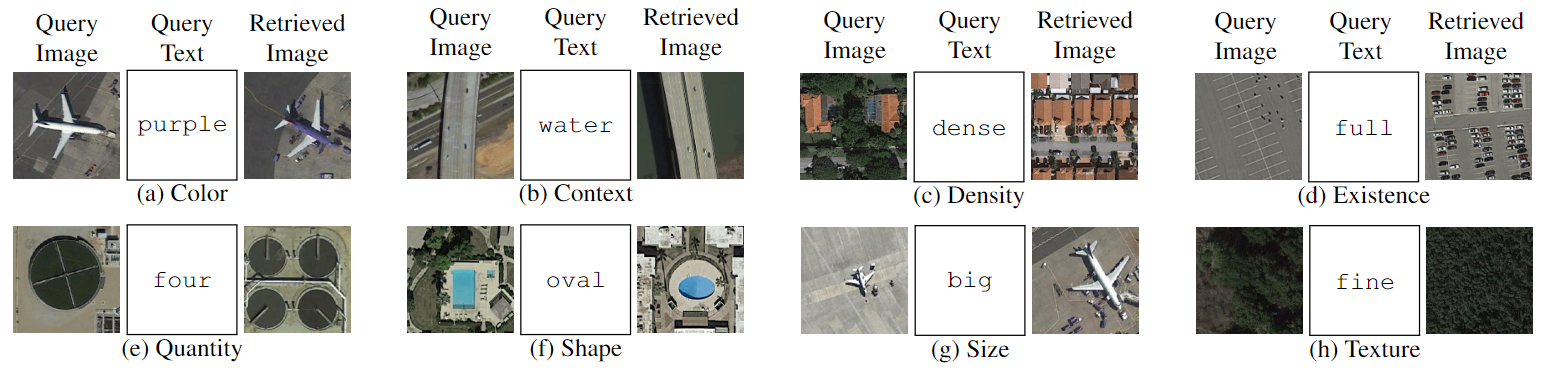
\includegraphics[width=\textwidth]{images/relatedworks/attr_use_cases_v2.png}
\caption{The eight attribute use cases covered by PATTERNCOM: color, context, density, existence, quantity, shape, size, and texture. Each query pairs a reference image with an attribute-modifying text and must retrieve an image of the same class exhibiting the target attribute value; subfigures (b) and (d) extend this to queries spanning multiple classes and attributes. Adapted from \cite{psomas2024composed}.}
\label{fig:rw-patterncom-attrs}
\end{figure}
 
Table~\ref{tab:rw-retrieval-datasets} summarizes the retrieval datasets and benchmarks discussed in this section, positioned along the unimodal-to-composed-to-temporal axis that leads to CTCR-RS.

\begin{table}[h]
\centering
\small
\begin{tabularx}{\textwidth}{l X c c}
\hline
\textbf{Name} & \textbf{Task / query type} & \textbf{Modalities} & \textbf{\# Images / pairs} \\
\hline
RSICD~\cite{lu2017exploring} & Image-text retrieval & Optical (RGB) & 10,921 \\
RSITMD~\cite{yuan2022exploring} & Image-text retrieval (fine-grained) & Optical (RGB) & 4,743 \\
PatternNet~\cite{zhou2018patternnet} & Image-image retrieval & Optical (RGB) & 30,400 \\
CIRR~\cite{liu2021cirr} & Composed image retrieval (natural images) & Optical (RGB) & 21,552 images, 36,554 triplets \\
FashionIQ~\cite{wu2021fashioniq} & Composed image retrieval (fashion) & Optical (RGB) & 77,684 images, 60,272 triplets \\
WebVid-CoVR~\cite{ventura2024covr} & Composed video retrieval, auto-mined & Video & 1.6M triplets \\
PATTERNCOM~\cite{psomas2024composed} & Composed image retrieval (image + text) & Optical (RGB) & 21,000+ queries \\
CTCR-RS (this thesis) & Composed temporal change retrieval (bi-temporal images + text) & Optical / SAR & 30,179 triplets \\
\hline
\end{tabularx}
\caption{Image-text, composed, and temporal retrieval datasets, from general-domain benchmarks (CIRR, FashionIQ, WebVid-CoVR) to remote sensing (RSICD, RSITMD, PatternNet, PATTERNCOM) and CTCR-RS.}
\label{tab:rw-retrieval-datasets}
\end{table}

\subsection{Methods for composed retrieval}
\label{sec:rw-retrieval-methods}

Outside RS, most CIR methods share a common architecture: a composition module fuses the reference image embedding and the modification text embedding into a single composed query embedding, which is then compared against candidate image embeddings via a contrastive objective, so that the composed embedding lands close to the target image and far from distractors. TIRG~\cite{vo2018composingtextimageimage} is an early example of this design, gating and residually combining image and text features rather than simply concatenating or averaging them. WEICOM, discussed next, departs from this paradigm entirely by avoiding a learned combiner altogether.

Composed image retrieval (CIR) was introduced to RS by \textcite{psomas2024composed} together with the PATTERNCOM benchmark above. Their method, WEICOM, is training-free: it fuses image-to-image and text-to-image similarities from a frozen VLM (CLIP or RemoteCLIP, discussed further in Section~\ref{sec:rw-foundation}) via a modality control parameter $\lambda$ that controls the relative weight given to the image and text parts of the query, avoiding the need for supervised composed-retrieval triplets that are costly to annotate at scale. This training-free design directly addresses the annotation bottleneck that motivated CoVR in the general vision-language literature, though via a different mechanism: WEICOM sidesteps the need for triplets altogether by fusing similarities at inference time, whereas CoVR sidesteps manual annotation by mining triplets automatically and still trains a dedicated combiner-style model. Follow-up work benchmarks composed retrieval specifically for applied EO use cases~\cite{efthymiadis2026benchmarking}, further establishing CIR as a distinct evaluation setting in RS beyond this initial benchmark.

PATTERNCOM's composed query, however, operates on a single, static image: the text modifies an attribute of a scene that does not itself change over time. This thesis' CTCR-RS contribution extends composed retrieval to the temporal setting: the reference is a bi-temporal image pair already exhibiting some change, and the text specifies an additional, compositional change to be added, with the target being a bi-temporal pair exhibiting the combined change. This is close in spirit to self-supervised cross-modal text-image time series retrieval~\cite{vuran2025selfsupervised}, which also moves retrieval toward multi-temporal image series, though without the compositional image-plus-text query structure that defines CIR. CTCR-RS can thus be read as the temporal, compositional counterpart to PATTERNCOM's attribute-based composed query, applied to the task of retrieving land-use and land-cover change rather than static scene attributes.

\subsection{Evaluating retrieval and composed retrieval}
\label{sec:rw-retrieval-metrics}

Retrieval, composed or otherwise, is evaluated with ranking metrics rather than classification accuracy, since the system returns a ranked list of candidates rather than a single answer. Recall@K (most commonly K = 1, 5, 10) reports the proportion of queries for which the correct target appears within the top-K retrieved candidates, and is the standard metric across RSICD, RSITMD, CIRR, FashionIQ, and PATTERNCOM alike. CIRR additionally reports a fine-grained Recall@K restricted to a small subset of visually similar distractors per query, specifically to prevent models from succeeding via coarse visual similarity alone rather than genuinely reasoning about the modification text. Mean or median rank of the correct target is sometimes reported alongside Recall@K, particularly when the candidate gallery is large enough that top-K recall alone saturates or fails to distinguish strong from weak retrieval quality. For CTCR-RS, the temporal, compositional nature of the query makes this distinction between coarse visual similarity and genuine change-reasoning especially relevant, echoing CIRR's fine-grained evaluation motivation above.

\subsection{Open challenges in composed retrieval}
\label{sec:rw-retrieval-challenges}

Composed retrieval in RS faces two open challenges directly relevant to this thesis. \textbf{Data scarcity}: unlike general-domain CIR, which benefits from automatically mined resources at the million-triplet scale (WebVid-CoVR~\cite{ventura2024covr}), RS composed retrieval still relies on a single, manually constructed benchmark (PATTERNCOM); no equivalent large-scale, automatically mined RS composed-retrieval resource yet exists, which likely limits how well WEICOM-style training-free methods and future learned combiners can be evaluated at scale. \textbf{Extending composition beyond static attributes}: PATTERNCOM's composed queries modify a single static attribute of a single-instant scene; extending composed retrieval to multi-temporal, multi-sensor settings, as CTCR-RS does, or to other forms of composition (e.g. compositional change across three or more time steps rather than two) remains largely unexplored.

\section{Captioning}
\label{sec:rw-captioning}

Image captioning is not a standalone contribution of this thesis; it appears as one component of a multi-task study alongside RSVQA and image reconstruction (Chapter~\ref{chap:multitask}). This section therefore does not survey RS captioning as a field in its own, but focuses on how captioning and RSVQA have been combined, either as a shared multi-task objective or as an intermediate mechanism within a VQA pipeline, since this is the angle relevant to the thesis' contribution.

\subsection{Datasets for joint captioning and RSVQA}
\label{sec:rw-captioning-datasets}

Datasets specifically built to support joint captioning-and-VQA study remain limited. RSICap~\cite{hu2023rsgpt} was introduced alongside RSGPT to provide long-form, detailed human-annotated captions suited to instruction-tuned VLMs, and is used by RSGPT for joint captioning and VQA fine-tuning. RS-Instructions, introduced alongside RS-LLaVA~\cite{diallo2024rsllava}, takes a different approach: rather than collecting new annotations, it combines four existing single-task captioning and VQA datasets (including UCM-Captions and RSVQA-LR) into a single multi-task instruction-tuning corpus. The underlying assumption is that joint training on this combined data improves general RS understanding more than task-specific fine-tuning would.

\subsection{Models coupling captioning and RSVQA}
\label{sec:rw-captioning-models}

Captioning and RSVQA have been coupled in the literature in two distinct ways. The first uses captioning-style image description as an interpretability step inside the VQA pipeline itself, rather than as an end task. Prompt-RSVQA~\cite{chappuis2022promptrsvqa} converts the image into a short textual description and feeds it, together with the question, to a language model, effectively delegating the visual grounding step to a captioning-like module before reasoning. MT-prompt-RSVQA~\cite{chappuis2023multitask} extends this by enriching the description with additional semantic information (land-cover classes, detected object counts) and by explicitly supervising an auxiliary counting objective, optimized jointly with the main VQA loss during training rather than handled by a separate, frozen pipeline step. PAN-RSVQA~\cite{chappuis2025pan} generalizes the idea further, using a vision foundation model to produce several pseudo-annotations (classification, segmentation, detection, generic features) jointly consumed by a multi-modal transformer; the visual description function that a captioning model would otherwise fill is here distributed across several pseudo-annotation streams.

The second family treats captioning and VQA as two supervised outputs of a single shared model, trained jointly on blended datasets rather than one task feeding the other. RS-LLaVA~\cite{diallo2024rsllava} adapts LLaVA to RS imagery via LoRA fine-tuning on the RS-Instructions dataset described above. In a related but architecturally different setting, a UAV aerial video model~\cite{uav2024videocaptioning} explicitly chains the two tasks, inserting a VQA step before the captioning decoder so that the answers to solicited questions enrich the information available for caption generation, an ordering that is the mirror image of Prompt-RSVQA's caption-then-answer pipeline.

These two families illustrate the two ways captioning and VQA have been coupled in the literature: captioning (or a captioning-like description) as an intermediate representation feeding VQA reasoning (Prompt-RSVQA, MT-prompt-RSVQA, PAN-RSVQA), and captioning and VQA as jointly supervised, parallel outputs of a shared model (RS-LLaVA, the UAV video model). The multi-task study in Chapter~\ref{chap:multitask} sits closer to the second family, but adds image reconstruction as a third, self-supervised objective alongside VQA and captioning, which neither of the above considers. Larger, task-agnostic VLMs that also cover captioning and VQA among several other capabilities (e.g. RSGPT, GeoChat) are discussed in Section~\ref{sec:rw-foundation}.

\subsection{Evaluating captioning alongside RSVQA}
\label{sec:rw-captioning-metrics}

Captioning is conventionally evaluated with n-gram overlap metrics borrowed from machine translation and general-domain captioning: BLEU measures precision of overlapping n-grams against reference captions, ROUGE measures recall-oriented overlap, and METEOR additionally accounts for synonymy and stemming; CIDEr, designed specifically for captioning, weights n-grams by their TF-IDF specificity so that generic, uninformative phrases contribute less to the score than distinctive ones. All four remain standard on NWPU-Captions, RSICD, and related benchmarks. These metrics, however, rely on surface-form overlap with a fixed set of reference captions and penalize a semantically correct but differently-worded caption. As discussed for VQA (Section~\ref{sec:rw-vqa-metrics}), this thesis' evaluation methodology adopts BERTScore~\cite{zhang2020bertscoreevaluatingtextgeneration} for its multi-task study, applying the same embedding-based similarity metric to both the captioning and VQA outputs of the shared model, which allows a single evaluation methodology to cover both tasks, reported alongside accuracy for VQA and ROUGE-1/ROUGE-L for captioning.

\subsection{Open challenges in joint captioning and RSVQA}
\label{sec:rw-captioning-challenges}

The main open challenge specific to the captioning-and-VQA setting reviewed in this section is that joint training is consistently motivated by an assumed synergy between tasks, but that synergy is rarely measured directly, and where it is measured, the evidence is mixed rather than confirmatory: RS-LLaVA's own reported results show single-task fine-tuning outperforming joint training on both captioning and VQA metrics, directly contradicting the premise behind combining the two tasks in RS-Instructions. Prompt-RSVQA-style approaches treat a captioning-like description as beneficial to VQA reasoning by construction, but in each case the improvement is attributed to the combination as a whole rather than isolated per task: it remains unclear how much of the gain comes specifically from captioning, how much from VQA, and how the two interact when a third objective is added. This thesis' multi-task study (Chapter~\ref{chap:multitask}) addresses this directly by ablating each task, training RSVQA, captioning, and image reconstruction jointly, to measure the specific contribution of each task to the others rather than assuming it. A related, more general challenge is the tension between the short, template-derived captions typical of automatically generated RS captioning data and the longer, richer descriptions that better support a VQA-style reasoning objective when the two tasks are trained jointly; datasets such as RSICap that provide long-form, human-written captions specifically for instruction-tuned VLMs are one response to this tension, but at the cost of scale relative to automatically annotated alternatives.
\section{Task-agnostic models and foundation models}
\label{sec:rw-foundation}

The families reviewed above are largely task-specific: an architecture designed for RSVQA, for CIR, or for captioning. A separate and increasingly dominant line of work instead builds a single RS-adapted model intended to handle several of these tasks at once, typically by adapting a pretrained large language model (LLM) or contrastive vision-language model to RS imagery. This section reviews these task-agnostic models, split into instruction-tuned generative VLMs and contrastive foundation encoders.

\textbf{Instruction-tuned generative VLMs.} RSGPT~\cite{hu2023rsgpt} fine-tunes an LLM-based VLM specifically for RS image understanding using the RSICap dataset (Section~\ref{sec:rw-captioning-datasets}), reporting gains on both captioning and VQA from joint instruction tuning. GeoChat~\cite{kuckreja2024geochat} extends this to grounded, region-level question answering. LHRS-Bot~\cite{muhtar2025lhrsbot} and its improved successor LHRS-Bot-Nova incorporate volunteered geographic information to strengthen visual-linguistic grounding, while SkyEyeGPT~\cite{zhan2025skyeyegpt} unifies several RS vision-language tasks, including VQA, through instruction tuning. EarthGPT~\cite{zhang2024earthgpt} processes SAR, optical, and infrared inputs jointly through a cross-modal comprehension module, extending capability beyond optical imagery within a single unified model.

More recent unified models push further toward multi-task, multi-sensor coverage: SkySenseGPT~\cite{luo2024skysensegptfinegrainedinstructiontuning} builds on the SkySense foundation model with fine-grained instruction tuning for vision-language understanding, RSUniVLM~\cite{liu2024rsunivlmunifiedvisionlanguage} and GeoRSMLLM~\cite{zhang2025georsmllmmultimodallargelanguage} adopt mixture-of-experts or unified architectures spanning multiple granularities of RS vision-language tasks, and TEOChat~\cite{irvin2025teochatlargevisionlanguageassistant} and UniRS~\cite{li2024unirsunifyingmultitemporalremote} specifically target temporal RS data, extending question answering to multi-temporal image series rather than single acquisitions. This temporal extension is directly relevant to the composed temporal retrieval setting this thesis addresses in Chapter~\ref{chap:ctcr}, even though these models target question answering rather than retrieval. A recurring limitation across this family, already noted in the RSVQA literature specifically~\cite{boussaidtosato2025tour}, is that most of these generative VLMs report strong results on descriptive or classification-style questions but rarely publish detailed results on the numerical questions that RSVQA datasets, which limits fair comparison against the task-specific classification-based baselines discussed in Section~\ref{sec:rw-vqa-methods}.

\textbf{Contrastive foundation encoders.} A separate, encoder-only line of work adapts CLIP-style contrastive pretraining to RS imagery, producing a general-purpose visual-textual embedding space rather than a generative decoder. RemoteCLIP~\cite{liu2024remoteclip} is the reference model in this family and is used directly as the frozen encoder backbone in WEICOM (Section~\ref{sec:rw-retrieval-methods}). RS5M and GeoRSCLIP~\cite{zhang2024rs5m} scale this pretraining to a larger RS image-text corpus, and more recent encoders such as DGTRS-CLIP~\cite{chen2025dgtrsddgtrsclipdualgranularity}, which targets dual-granularity alignment, continue this line of work. All of these report unimodal image-text retrieval performance as a core evaluation of alignment quality, and any of them could in principle serve as the frozen encoder backbone for a WEICOM-style composed retrieval method, though to date only CLIP and RemoteCLIP have been evaluated in that specific composed setting. Because these encoders are trained without any task-specific supervision, they are equally applicable to retrieval, zero-shot classification, and as a visual encoder for VQA or captioning models, making them the clearest instance of the task-agnostic framing that motivates this section.

\section{Positioning of this thesis}
\label{sec:rw-positioning}
 
The landscape reviewed in this chapter is where this thesis' five contributions fit. The first three sit within RSVQA specifically (Section~\ref{sec:rw-vqa}). A data augmentation strategy targets the training-strategy dimension reviewed in Section~\ref{sec:rw-vqa-methods}. Segmentation-guided attention uses image segmentation to focus the model's attention on question-relevant regions, one of the interpretability mechanisms discussed under image processing in Section~\ref{sec:rw-vqa-methods}. TAMMI/MM-RSVQA addresses the multi-modality challenge identified in Section~\ref{sec:rw-vqa-challenges} directly, by fusing very high-resolution optical imagery with SAR and multispectral data rather than optical imagery alone.

The remaining two contributions extend this RSVQA foundation outward, each into one of the other two tasks reviewed in this chapter. Unlike PATTERNCOM, which relies on manual triplet annotation, CTCR-RS is built by extracting change labels automatically from existing change captinoing datasets, closer to the automatic-construction of CoVR than to PATTERNCOM's manual annotation, even though the underlying mechanism differs. No prior RS dataset or method extends composition beyond static attributes to compositional, multi-temporal change. The multi-task study (Section~\ref{sec:rw-captioning}) instead connects RSVQA to two other tasks in a different way, training RSVQA jointly with captioning and image reconstruction and directly addressing the open challenge identified in Section~\ref{sec:rw-captioning-challenges}: rather than assuming a synergy between jointly trained tasks that goes unmeasured, or, as in RS-LLaVA's own results, contradicted, it isolates the contribution of each task through systematic ablation across every task combination.
 
This progression is not a coincidence: RS vision-language research began with  task-specific architectures for RSVQA, captioning, and retrieval studied largely in isolation, and is increasingly moving toward models and methods that treat these tasks, and the synergies between them, together rather than as three separate problems (Section~\ref{sec:rw-foundation}). The remaining chapters detail each of the five contributions in turn.